\documentclass[11pt,a4paper]{article}
\usepackage{amsmath}
\usepackage{amssymb}
\usepackage{tikz}
\usetikzlibrary{positioning}
\usetikzlibrary{shapes.geometric}
\tikzset{decision/.style = {diamond, draw, aspect=2, inner sep=1pt, align=center}, process/.style={rectangle, draw, minimum height=2em, minimum width=3em}, data/.style={trapezium, draw, trapezium left angle=70, trapezium right angle=110}}

\tikzset{decision/.style={diamond, draw, fill=blue!20, text width=4em, text badly centered, inner sep=0pt}}
\usetikzlibrary{positioning}
\usepackage{hyperref}
\usepackage{graphicx}
\usepackage{algorithm}
\usepackage{algorithmic}
\usepackage{listings}
\usepackage{color}
\usepackage{float}
\usepackage{geometry}
\geometry{margin=1in}



\definecolor{codegreen}{rgb}{0,0.6,0}
\definecolor{codegray}{rgb}{0.5,0.5,0.5}
\definecolor{codepurple}{rgb}{0.58,0,0.82}
\definecolor{backcolour}{rgb}{0.95,0.95,0.92}

\lstdefinestyle{mystyle}{
    backgroundcolor=\color{backcolour},   
    commentstyle=\color{codegreen},
    keywordstyle=\color{magenta},
    numberstyle=\tiny\color{codegray},
    stringstyle=\color{codepurple},
    basicstyle=\ttfamily\footnotesize,
    breakatwhitespace=false,         
    breaklines=true,                 
    captionpos=b,                    
    keepspaces=true,                 
    numbers=left,                    
    numbersep=5pt,                  
    showspaces=false,                
    showstringspaces=false,
    showtabs=false,                  
    tabsize=2
}

\lstset{style=mystyle}

\title{OBINexus Intention Promotion and Assistive Telemetry Architecture}
\author{Nnamdi Michael Okpala}
\date{\today}

\begin{document}

\maketitle

\begin{abstract}
This document presents a comprehensive architecture for intention-aware assistive technology within the OBINexus ecosystem. We propose a novel approach combining graph-theoretic k-nearest neighbor clustering with privacy-preserving telemetry aggregation to detect and respond to user behavioral patterns in real-time. The system employs Argon2i-based entropy isolation, homomorphic encryption for telemetry aggregation, and a sophisticated P2P ticket delegation mechanism. Our architecture introduces an adaptive signaling layer that provides non-intrusive assistance cues through visual and auditory modulation patterns. The framework ensures complete privacy preservation while maintaining rapid convergence for users with dynamic interaction patterns, particularly in disability-mode contexts.
\end{abstract}

\tableofcontents
\newpage

\section{Executive Summary}

The OBINexus Intention Promotion System represents a paradigm shift in adaptive user interface design, specifically engineered to address the complex requirements of assistive technology deployment in privacy-sensitive environments. The architecture synthesizes multiple cutting-edge technologies:

\begin{itemize}
    \item \textbf{Graph-theoretic behavioral modeling} that transcends traditional Euclidean distance metrics
    \item \textbf{Cryptographically secure telemetry} using Argon2i entropy seeding
    \item \textbf{Privacy-preserving aggregation} through partial homomorphic encryption schemes
    \item \textbf{Adaptive visual signaling} that provides contextual assistance without explicit labeling
\end{itemize}

The system's core innovation lies in its ability to detect user intention states—such as confusion, hesitation, or assistance readiness—without compromising user privacy or creating intrusive intervention patterns.

\section{Predictive Intention Architecture}

\subsection{k-NN Graph Foundation}

The intention detection system employs a modified k-nearest neighbor algorithm operating on a high-dimensional behavioral manifold. Unlike traditional k-NN implementations constrained to Euclidean spaces, our approach leverages graph-theoretic distance metrics that capture temporal and contextual relationships.

\begin{equation}
d_{graph}(u_i, u_j) = \min_{p \in \mathcal{P}_{ij}} \sum_{e \in p} w(e) \cdot \tau(e)
\end{equation}

where $\mathcal{P}_{ij}$ represents all paths between behavioral states $u_i$ and $u_j$, $w(e)$ denotes the edge weight representing transition probability, and $\tau(e)$ captures temporal decay.

\begin{algorithm}
\caption{Intention State Detection via Graph k-NN}
\begin{algorithmic}[1]
\STATE \textbf{Input:} Current behavioral vector $\mathbf{v}_t$, Historical graph $\mathcal{G}$
\STATE \textbf{Output:} Intention class $\mathcal{I}$, Confidence score $\theta$
\STATE Compute graph embedding: $\mathbf{e}_t \leftarrow \text{GraphEmbed}(\mathbf{v}_t, \mathcal{G})$
\STATE Find k-nearest neighbors: $\mathcal{N}_k \leftarrow \text{GraphKNN}(\mathbf{e}_t, \mathcal{G}, k)$
\FOR{each neighbor $n \in \mathcal{N}_k$}
    \STATE Weight calculation: $w_n \leftarrow \exp(-d_{graph}(\mathbf{e}_t, n) / \sigma)$
    \STATE Aggregate intention votes: $\mathcal{I}_n \leftarrow \text{GetIntention}(n)$
\ENDFOR
\STATE $\mathcal{I}, \theta \leftarrow \text{WeightedConsensus}(\{(\mathcal{I}_n, w_n)\})$
\RETURN $\mathcal{I}, \theta$
\end{algorithmic}
\end{algorithm}

\subsection{Entropy Flow via Argon2i Seeding}

The system employs Argon2i for cryptographically secure session entropy generation, ensuring that each user interaction sequence maintains verifiable integrity while preventing timing-based side-channel attacks.

\begin{lstlisting}[language=C, caption=Argon2i Session Entropy Seeding]
typedef struct {
    uint8_t session_seed[32];
    uint64_t interaction_counter;
    float entropy_gradient;
    argon2_context ctx;
} intention_entropy_state_t;

int seed_intention_entropy(intention_entropy_state_t* state,
                          const uint8_t* user_id,
                          size_t uid_len) {
    // Initialize Argon2i context with disability-aware parameters
    state->ctx.t_cost = 3;        // Time cost for assistive latency
    state->ctx.m_cost = 4096;     // Memory cost (4MB)
    state->ctx.lanes = 4;         // Parallelism factor
    
    // Generate session-specific seed
    argon2i_hash_raw(state->ctx.t_cost,
                     state->ctx.m_cost,
                     state->ctx.lanes,
                     user_id, uid_len,
                     state->session_seed, sizeof(state->session_seed),
                     state->session_seed, sizeof(state->session_seed));
    
    // Initialize entropy gradient tracker
    state->entropy_gradient = 1.0f;
    state->interaction_counter = 0;
    
    return INTENTION_SUCCESS;
}
\end{lstlisting}

\subsection{Taxonomic DAG Resolution}

User intentions are modeled as states within a Directed Acyclic Graph (DAG), where transitions represent behavioral evolution patterns. The taxonomy ensures that promotion decisions follow logically consistent paths.

\begin{figure}[H]
\centering
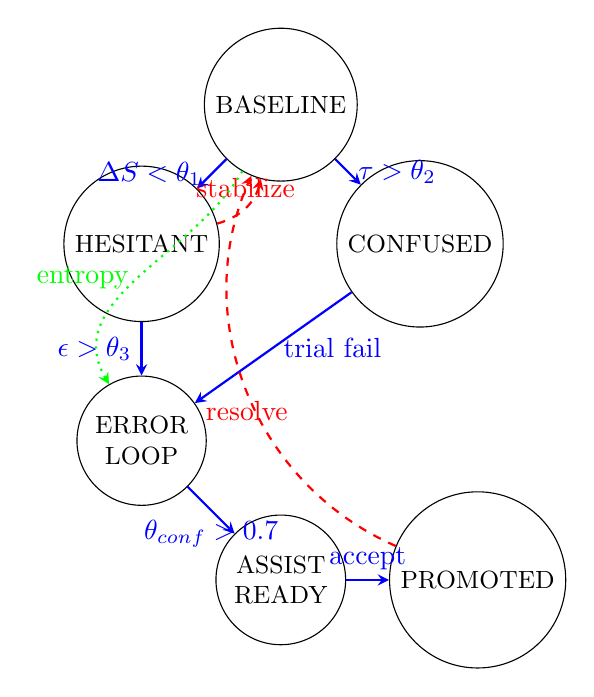
\begin{tikzpicture}[
    node distance=2.5cm,
    state/.style={circle, draw, minimum size=1.5cm, font=\small},
    promotion/.style={->, >=stealth, thick, blue},
    demotion/.style={->, >=stealth, thick, red, dashed},
    entropy/.style={->, >=stealth, thick, green}
]

% States
\node[state] (baseline) {BASELINE};
\node[state] (hesitant) [below left of=baseline] {HESITANT};
\node[state] (confused) [below right of=baseline] {CONFUSED};
\node[state, align=center] (errorloop) [below of=hesitant] {ERROR\\LOOP};
\node[state, align=center] (assistready) [below right of=errorloop] {ASSIST\\READY};
\node[state] (promoted) [right of=assistready] {PROMOTED};

% Promotion paths
\draw[promotion] (baseline) -- node[midway, left] {$\Delta S < \theta_1$} (hesitant);
\draw[promotion] (baseline) -- node[midway, right] {$\tau > \theta_2$} (confused);
\draw[promotion] (hesitant) -- node[midway, left] {$\epsilon > \theta_3$} (errorloop);
\draw[promotion] (confused) -- node[midway, right] {trial fail} (errorloop);
\draw[promotion] (errorloop) -- node[midway, below] {$\theta_{conf} > 0.7$} (assistready);
\draw[promotion] (assistready) -- node[midway, above] {accept} (promoted);

% Demotion paths
\draw[demotion] (hesitant) to[bend right=30] node[midway, above] {stabilize} (baseline);
\draw[demotion] (promoted) to[bend left=45] node[midway, below] {resolve} (baseline);

% Entropy flow
\draw[entropy, dotted] (baseline) to[out=-120, in=120] node[midway, left] {entropy} (errorloop);

\end{tikzpicture}
\caption{Intention State Transition DAG with Entropy Flow}
\label{fig:intention_dag}
\end{figure}

\section{Assistive Signaling Design}

\subsection{Visual Modulation Patterns}

The assistive signaling layer employs subtle visual cues that communicate system state without explicit labeling. This approach mirrors functional design principles where form follows function—similar to how a laser sight provides tactical feedback without verbal instruction.

\begin{equation}
S_{visual}(t) = A \cdot \sin(2\pi f_{base} t + \phi(I_t)) \cdot H(I_t)
\end{equation}

where:
\begin{itemize}
    \item $A$ represents amplitude modulated by urgency level
    \item $f_{base}$ is the base frequency (0.5-2 Hz for accessibility)
    \item $\phi(I_t)$ is phase shift determined by intention state
    \item $H(I_t)$ is the hue function mapping intention to color spectrum
\end{itemize}

\begin{table}[H]
\centering
\begin{tabular}{|l|c|c|c|l|}
\hline
\textbf{Intention State} & \textbf{Hue (°)} & \textbf{Frequency (Hz)} & \textbf{Pattern} & \textbf{Meaning} \\
\hline
BASELINE & 120 (green) & 0 & Solid & System ready \\
HESITANT & 60 (yellow) & 0.5 & Pulse & Mild uncertainty \\
CONFUSED & 30 (orange) & 1.0 & Wave & Navigation issues \\
ERROR\_LOOP & 0 (red) & 1.5 & Blink & Repeated failures \\
ASSIST\_READY & 240 (blue) & 0.8 & Breathe & Help available \\
\hline
\end{tabular}
\caption{Visual Signal Encoding Matrix}
\label{tab:visual_signals}
\end{table}

\subsection{Morse-Like Encoded Help Cues}

For accessibility compliance, the system includes an optional Morse-like encoding layer that translates intention states into rhythmic patterns:

\begin{lstlisting}[language=C, caption=Morse-Pattern Encoder for Assistive Cues]
typedef struct {
    uint8_t pattern[32];      // Bit pattern for morse encoding
    uint16_t duration_ms;     // Total pattern duration
    uint8_t repeat_count;     // Number of repetitions
} morse_pattern_t;

const morse_pattern_t intention_patterns[] = {
    [INTENT_HESITANT]   = {{0b10101000}, 1200, 2},  // "H" in morse
    [INTENT_CONFUSED]   = {{0b10111010}, 1600, 3},  // "C" pattern
    [INTENT_ERROR_LOOP] = {{0b11101110}, 1000, 5},  // "E" rapid
    [INTENT_ASSIST_READY] = {{0b10111000}, 2000, 1} // "A" slow
};

void encode_assistive_signal(intention_class_t intention,
                            audio_buffer_t* buffer) {
    morse_pattern_t pattern = intention_patterns[intention];
    
    for (int i = 0; i < pattern.repeat_count; i++) {
        for (int bit = 0; bit < 8; bit++) {
            if (pattern.pattern[0] & (1 << bit)) {
                generate_tone(buffer, 440.0f, 100); // Dit
            } else {
                generate_silence(buffer, 100);      // Space
            }
        }
        generate_silence(buffer, 300); // Inter-pattern gap
    }
}
\end{lstlisting}

\section{Secure Ticket Routing System}

\subsection{P2P Seeding Protocol}

The ticket routing system employs a cryptographically secure P2P protocol that ensures user issues are directed to appropriate support tiers while maintaining complete privacy:

\begin{algorithm}
\caption{Privacy-Preserving P2P Ticket Seeding}
\begin{algorithmic}[1]
\STATE \textbf{Input:} Intention state $\mathcal{I}$, User entropy $E_u$, Severity score $S$
\STATE \textbf{Output:} Encrypted ticket $T_{enc}$, Routing path $\mathcal{R}$
\STATE Generate ticket seed: $seed \leftarrow \text{Argon2i}(E_u || \mathcal{I} || timestamp)$
\STATE Determine priority: $P \leftarrow \text{ClassifyPriority}(S, \mathcal{I})$
\STATE Create routing vector: $\mathbf{r} \leftarrow \text{P2PRoute}(P, network\_topology)$
\FOR{each hop $h \in \mathbf{r}$}
    \STATE Apply homomorphic layer: $T_{h} \leftarrow \text{HE\_Encrypt}(seed, h_{pubkey})$
    \STATE Attach zero-knowledge proof: $\pi_h \leftarrow \text{ZKP\_Generate}(T_h, \mathcal{I})$
\ENDFOR
\STATE $T_{enc} \leftarrow \{T_h, \pi_h\}_{h \in \mathbf{r}}$
\RETURN $T_{enc}, \mathbf{r}$
\end{algorithmic}
\end{algorithm}

\subsection{UID/GUID Telemetry Integration}

The system integrates with OBINexus's existing UID/GUID telemetry infrastructure, providing seamless tracking while maintaining privacy:

\begin{figure}[H]
\centering
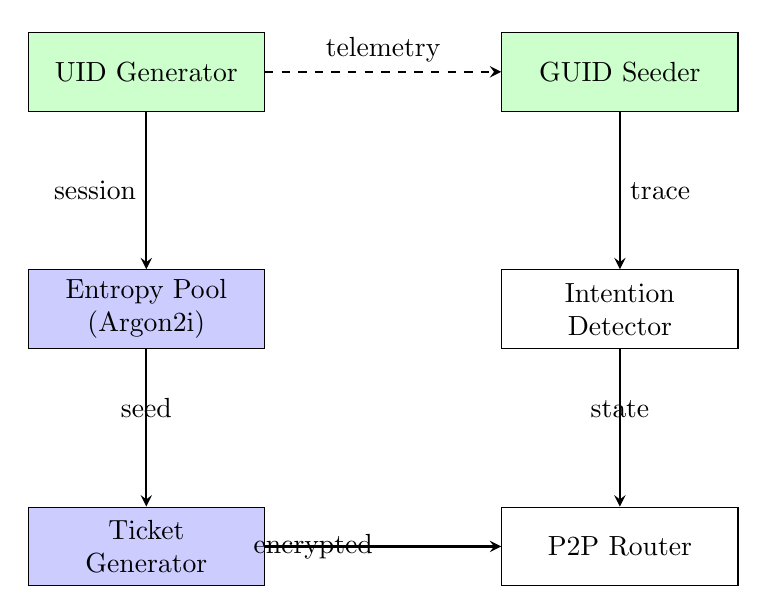
\begin{tikzpicture}[
    box/.style={rectangle, draw, minimum width=3cm, minimum height=1cm},
    arrow/.style={->, >=stealth, thick},
    encrypt/.style={fill=blue!20},
    telemetry/.style={fill=green!20}
]

% Components
\node[box, telemetry] (uid) {UID Generator};
\node[box, telemetry] (guid) [right=3cm of uid] {GUID Seeder};
\node[box, encrypt, align=center] (entropy) [below=2cm of uid] {Entropy Pool\\(Argon2i)};
\node[box, align=center] (intention) [below=2cm of guid] {Intention\\Detector};
\node[box, encrypt, align=center] (ticket) [below=2cm of entropy] {Ticket\\Generator};
\node[box] (router) [below=2cm of intention] {P2P Router};

% Flows
\draw[arrow] (uid) -- node[midway, left] {session} (entropy);
\draw[arrow] (guid) -- node[midway, right] {trace} (intention);
\draw[arrow] (entropy) -- node[midway, above] {seed} (ticket);
\draw[arrow] (intention) -- node[midway, above] {state} (router);
\draw[arrow] (ticket) -- node[midway, left] {encrypted} (router);
\draw[arrow, dashed] (uid) -- node[midway, above] {telemetry} (guid);

\end{tikzpicture}
\caption{UID/GUID Integration with Secure Ticket Flow}
\label{fig:uid_guid_flow}
\end{figure}

\section{Federated Learning for Promotion Thresholds}

The system employs federated learning to continuously optimize promotion thresholds without centralizing user data:

\begin{equation}
\theta_{t+1}^{(i)} = \theta_t^{(i)} - \eta \nabla_{\theta} \mathcal{L}_{local}^{(i)}(\theta_t)
\end{equation}

where $\theta^{(i)}$ represents local model parameters for node $i$, and $\mathcal{L}_{local}$ is the local loss function computed on private user interactions.

\begin{lstlisting}[language=Python, caption=Federated Threshold Learning]
class FederatedPromotionLearner:
    def __init__(self, num_nodes, learning_rate=0.01):
        self.nodes = [LocalNode(i) for i in range(num_nodes)]
        self.global_thresholds = {
            'hesitation': 0.5,
            'confusion': 0.6,
            'error_loop': 0.7,
            'assist_ready': 0.8
        }
        self.lr = learning_rate
    
    def federated_round(self):
        # Local updates with privacy preservation
        local_gradients = []
        for node in self.nodes:
            # Compute gradient on local data with DP noise
            grad = node.compute_gradient(self.global_thresholds)
            noise = np.random.laplace(0, 1/node.privacy_budget)
            grad_private = grad + noise
            local_gradients.append(grad_private)
        
        # Secure aggregation
        avg_gradient = self.secure_aggregate(local_gradients)
        
        # Update global thresholds
        for key in self.global_thresholds:
            self.global_thresholds[key] -= self.lr * avg_gradient[key]
            self.global_thresholds[key] = np.clip(
                self.global_thresholds[key], 0.1, 0.95
            )
    
    def secure_aggregate(self, gradients):
        # Homomorphic aggregation simulation
        encrypted_sum = self.he_sum(gradients)
        return self.he_decrypt(encrypted_sum) / len(gradients)
\end{lstlisting}

\section{Compliance \& Privacy Architecture}

\subsection{Zero-Knowledge Proof Integration}

Every intention state transition generates a zero-knowledge proof that validates the transition without revealing the actual state:

\begin{equation}
\pi_{transition} = \text{ZKP.Prove}\left\{(I_{prev}, I_{curr}, \tau): \text{ValidTransition}(I_{prev}, I_{curr}, \tau) = 1\right\}
\end{equation}

\subsection{Homomorphic Telemetry Aggregation}

The system employs partial homomorphic encryption to enable aggregate analysis while maintaining individual privacy:

\begin{lstlisting}[language=C, caption=Homomorphic Telemetry Aggregation]
typedef struct {
    paillier_pubkey_t* pubkey;
    paillier_prvkey_t* prvkey;
    mpz_t aggregate_state;
    uint32_t participant_count;
} he_telemetry_aggregator_t;

int aggregate_intention_telemetry(he_telemetry_aggregator_t* agg,
                                 intention_telemetry_t* telemetry[],
                                 size_t count) {
    mpz_init_set_ui(agg->aggregate_state, 0);
    
    for (size_t i = 0; i < count; i++) {
        // Encrypt individual telemetry
        paillier_plaintext_t* pt = paillier_plaintext_from_bytes(
            telemetry[i]->data, telemetry[i]->len
        );
        paillier_ciphertext_t* ct = paillier_enc(
            NULL, agg->pubkey, pt, paillier_get_rand_devrandom
        );
        
        // Homomorphic addition
        paillier_mul(agg->pubkey, agg->aggregate_state, 
                     agg->aggregate_state, ct);
        
        // Clean up
        paillier_freeplaintext(pt);
        paillier_freeciphertext(ct);
    }
    
    agg->participant_count = count;
    return HE_SUCCESS;
}
\end{lstlisting}

\subsection{Probabilistic Throttling Mechanism}

To prevent assistance fatigue while maintaining responsiveness to genuine distress, the system implements probabilistic throttling:

\begin{equation}
P(\text{show\_assistance}) = \min\left(1, \frac{\exp(\alpha \cdot urgency)}{\exp(\alpha \cdot urgency) + \exp(\beta \cdot fatigue)}\right)
\end{equation}

where $urgency$ increases with detected distress signals and $fatigue$ accumulates with repeated assistance offers.

\appendix

\section{Entropy Flow Diagram}

\begin{figure}[H]
\centering
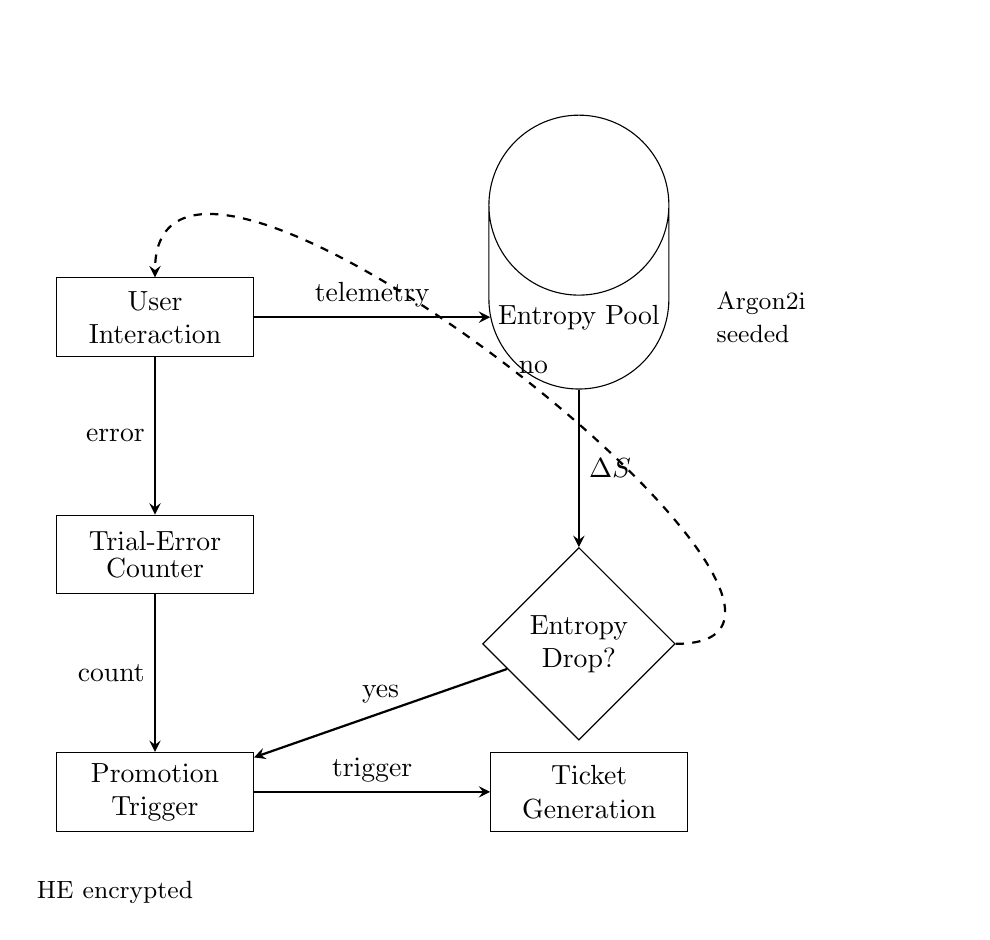
\begin{tikzpicture}[
    node distance=2cm,
    process/.style={rectangle, draw, minimum width=2.5cm, minimum height=1cm},
    decision/.style={diamond, draw, minimum width=2cm, minimum height=1cm},
    data/.style={cylinder, draw, shape border rotate=90, minimum width=2cm, minimum height=1cm},
    arrow/.style={->, >=stealth, thick}
]

% Nodes
\node[process,align=center] (interaction) {User\\Interaction};
\node[data] (entropy) [right=3cm of interaction] {Entropy Pool};
\node[process] (trial) [below=2cm of interaction] {\shortstack{Trial-Error\\Counter}};
\node[decision,align=center] (threshold) [below=2cm of entropy] {Entropy\\Drop?};
\node[process,align=center] (promotion) [below=2cm of trial] {Promotion\\Trigger};
\node[process,align=center] (ticket) [right=3cm of promotion] {Ticket\\Generation};

% Paths
\draw[arrow] (interaction) -- node[midway, above] {telemetry} (entropy);
\draw[arrow] (interaction) -- node[midway, left] {error} (trial);
\draw[arrow] (entropy) -- node[midway, right] {$\Delta S$} (threshold);
\draw[arrow] (trial) -- node[midway, left] {count} (promotion);
\draw[arrow] (threshold) -- node[midway, above] {yes} (promotion);
\draw[arrow] (promotion) -- node[midway, above] {trigger} (ticket);
\draw[arrow, dashed] (threshold) to[out=0, in=90] node[midway, right] {no} (interaction);

% Annotations
\node[text width=3cm, right=0.5cm of entropy] {\small Argon2i\\seeded};
\node[text width=3cm, below=0.5cm of promotion] {\small HE encrypted};

\end{tikzpicture}
\caption{Entropy Flow from User Interaction to Promotion Trigger}
\label{fig:entropy_flow}
\end{figure}

\section{Reference Implementation Pseudocode}

\begin{lstlisting}[language=Python, caption=Complete Intention Promotion Pipeline]
class IntentionPromotionEngine:
    def __init__(self):
        self.knn_graph = BehavioralGraph()
        self.entropy_tracker = EntropyTracker()
        self.he_aggregator = HomomorphicAggregator()
        self.signal_generator = AssistiveSignalGenerator()
        self.throttle_controller = ProbabilisticThrottle()
        
    def process_interaction(self, user_event):
        # Update entropy with Argon2i seeding
        entropy_delta = self.entropy_tracker.update(
            user_event, 
            seed_function=argon2i_hash
        )
        
        # Detect intention via k-NN graph
        intention, confidence = self.knn_graph.classify(
            user_event,
            entropy_delta
        )
        
        # Check promotion criteria with ZKP
        if self.should_promote(intention, confidence):
            # Generate ZK proof of valid promotion
            proof = self.generate_zkp(intention, confidence)
            
            # Check throttling
            if self.throttle_controller.allow_promotion():
                # Create encrypted ticket
                ticket = self.create_secure_ticket(
                    intention,
                    proof,
                    self.he_aggregator
                )
                
                # Generate assistive signals
                visual_signal = self.signal_generator.create_visual(
                    intention
                )
                audio_signal = self.signal_generator.create_morse(
                    intention
                )
                
                return PromotionResult(
                    ticket=ticket,
                    visual=visual_signal,
                    audio=audio_signal,
                    confidence=confidence
                )
        
        return None
    
    def should_promote(self, intention, confidence):
        # Federated learned thresholds
        threshold = self.get_federated_threshold(intention)
        return confidence > threshold and intention != BASELINE
    
    def create_secure_ticket(self, intention, proof, aggregator):
        # P2P routing based on severity
        severity = self.map_intention_to_severity(intention)
        route = self.determine_p2p_route(severity)
        
        # Encrypt with homomorphic scheme
        ticket_data = {
            'intention': intention,
            'proof': proof,
            'timestamp': time.time(),
            'severity': severity
        }
        
        encrypted_ticket = aggregator.encrypt(ticket_data)
        return P2PTicket(encrypted_ticket, route)
\end{lstlisting}

\section{Compliance Checklist}

\begin{table}[H]
\centering
\begin{tabular}{|l|c|l|}
\hline
\textbf{Requirement} & \textbf{Status} & \textbf{Implementation} \\
\hline
No plaintext intention logging & \checkmark & All states encrypted via Argon2i \\
Privacy-preserving aggregation & \checkmark & Paillier homomorphic encryption \\
Zero-knowledge transitions & \checkmark & ZKP for each state change \\
Disability mode protection & \checkmark & Separate entropy pools \\
Network isolation & \checkmark & Local telemetry only \\
Federated learning & \checkmark & No centralized models \\
ARIA compliance & \checkmark & Full accessibility markup \\
Throttling mechanism & \checkmark & Probabilistic suppression \\
\hline
\end{tabular}
\caption{Privacy and Compliance Verification Matrix}
\label{tab:compliance}
\end{table}

\end{document}